
\documentclass[a4paper,11pt]{article}
\usepackage[a4paper, margin=8em]{geometry}

% usa i pacchetti per la scrittura in italiano
\usepackage[french,italian]{babel}
\usepackage[T1]{fontenc}
\usepackage[utf8]{inputenc}
\frenchspacing 

% usa i pacchetti per la formattazione matematica
\usepackage{amsmath, amssymb, amsthm, amsfonts}

% usa altri pacchetti
\usepackage{gensymb}
\usepackage{hyperref}
\usepackage{standalone}

\usepackage{colortbl}

\usepackage{xstring}
\usepackage{karnaugh-map}

% imposta il titolo
\title{Electronics for Embedded Systems notes}
\author{Luca Seggiani}
\date{2026}

% spaziatura liste
\usepackage{enumitem}
\setlist[itemize]{noitemsep, topsep=4pt, partopsep=0pt, parsep=2pt, leftmargin=*}
\setlist[enumerate]{noitemsep, topsep=4pt, partopsep=0pt, parsep=2pt, leftmargin=*}

% imposta lo stile
% usa helvetica
\usepackage[scaled]{helvet}
% usa palatino
\usepackage{palatino}
% usa un font monospazio guardabile
\usepackage{lmodern}

\renewcommand{\rmdefault}{ppl}
\renewcommand{\sfdefault}{phv}
\renewcommand{\ttdefault}{lmtt}

% circuiti
\usepackage{circuitikz}
\usetikzlibrary{babel}

% testo cerchiato
\newcommand*\circled[1]{\tikz[baseline=(char.base)]{
            \node[shape=circle,draw,inner sep=2pt] (char) {#1};}}

% disponi il titolo
\makeatletter
\renewcommand{\maketitle} {
	\begin{center} 
		\begin{minipage}[t]{.8\textwidth}
			\textsf{\huge\bfseries \@title} 
		\end{minipage}%
		\begin{minipage}[t]{.2\textwidth}
			\raggedleft \vspace{-1.65em}
			\textsf{\small \@author} \vfill
			\textsf{\small \@date}
		\end{minipage}
		\par
	\end{center}

	\thispagestyle{empty}
	\pagestyle{fancy}
}
\makeatother

% disponi teoremi
\usepackage{tcolorbox}
\newtcolorbox[auto counter, number within=section]{theorem}[2][]{%
	colback=blue!10, 
	colframe=blue!40!black, 
	sharp corners=northwest,
	fonttitle=\sffamily\bfseries, 
	title=Theorem~\thetcbcounter: #2, 
	#1
}

% disponi definizioni
\newtcolorbox[auto counter, number within=section]{definition}[2][]{%
	colback=red!10,
	colframe=red!40!black,
	sharp corners=northwest,
	fonttitle=\sffamily\bfseries,
	title=Definition~\thetcbcounter: #2,
	#1
}

% disponi codice
\usepackage{listings}
\usepackage[table]{xcolor}

\definecolor{codegreen}{rgb}{0,0.6,0}
\definecolor{codegray}{rgb}{0.5,0.5,0.5}
\definecolor{codepurple}{rgb}{0.58,0,0.82}
\definecolor{backcolour}{rgb}{0.95,0.95,0.92}

\lstdefinestyle{codestyle}{
		backgroundcolor=\color{black!5}, 
		commentstyle=\color{codegreen},
		keywordstyle=\bfseries\color{magenta},
		numberstyle=\sffamily\tiny\color{black!60},
		stringstyle=\color{green!50!black},
		basicstyle=\ttfamily\footnotesize,
		breakatwhitespace=false,         
		breaklines=true,                 
		captionpos=b,                    
		keepspaces=true,                 
		numbers=left,                    
		numbersep=5pt,                  
		showspaces=false,                
		showstringspaces=false,
		showtabs=false,                  
		tabsize=2
}

\lstdefinestyle{shellstyle}{
		backgroundcolor=\color{black!5}, 
		basicstyle=\ttfamily\footnotesize\color{black}, 
		commentstyle=\color{black}, 
		keywordstyle=\color{black},
		numberstyle=\color{black!5},
		stringstyle=\color{black}, 
		showspaces=false,
		showstringspaces=false, 
		showtabs=false, 
		tabsize=2, 
		numbers=none, 
		breaklines=true
}

\lstdefinelanguage{x86}{ 
  keywords={AAA, AAD, AAM, AAS, ADC, ADCB, ADCW, ADCL, ADD, ADDB, ADDW, ADDL, AND, ANDB, ANDW, ANDL,
        ARPL, BOUND, BSF, BSFL, BSFW, BSR, BSRL, BSRW, BSWAP, BT, BTC, BTCB, BTCW, BTCL, BTR, 
        BTRB, BTRW, BTRL, BTS, BTSB, BTSW, BTSL, CALL, CBW, CDQ, CLC, CLD, CLI, CLTS, CMC, CMP,
        CMPB, CMPW, CMPL, CMPS, CMPSB, CMPSD, CMPSW, CMPXCHG, CMPXCHGB, CMPXCHGW, CMPXCHGL,
        CMPXCHG8B, CPUID, CWDE, DAA, DAS, DEC, DECB, DECW, DECL, DIV, DIVB, DIVW, DIVL, ENTER,
        HLT, IDIV, IDIVB, IDIVW, IDIVL, IMUL, IMULB, IMULW, IMULL, IN, INB, INW, INL, INC, INCB,
        INCW, INCL, INS, INSB, INSD, INSW, INT, INT3, INTO, INVD, INVLPG, IRET, IRETD, JA, JAE,
        JB, JBE, JC, JCXZ, JE, JECXZ, JG, JGE, JL, JLE, JMP, JNA, JNAE, JNB, JNBE, JNC, JNE, JNG,
        JNGE, JNL, JNLE, JNO, JNP, JNS, JNZ, JO, JP, JPE, JPO, JS, JZ, LAHF, LAR, LCALL, LDS,
        LEA, LEAVE, LES, LFS, LGDT, LGS, LIDT, LMSW, LOCK, LODSB, LODSD, LODSW, LOOP, LOOPE,
        LOOPNE, LSL, LSS, LTR, MOV, MOVB, MOVW, MOVL, MOVSB, MOVSD, MOVSW, MOVSX, MOVSXB,
        MOVSXW, MOVSXL, MOVZX, MOVZXB, MOVZXW, MOVZXL, MUL, MULB, MULW, MULL, NEG, NEGB, NEGW,
        NEGL, NOP, NOT, NOTB, NOTW, NOTL, OR, ORB, ORW, ORL, OUT, OUTB, OUTW, OUTL, OUTSB, OUTSD,
        OUTSW, POP, POPL, POPW, POPB, POPA, POPAD, POPF, POPFD, PUSH, PUSHL, PUSHW, PUSHB, PUSHA, 
        RCLL, RCR, RCRB, RCRW, RCRL, RDMSR, RDPMC, RDTSC, REP, REPE, REPNE, RET, ROL, ROLB, ROLW,
        ROLL, ROR, RORB, RORW, RORL, SAHF, SAL, SALB, SALW, SALL, SAR, SARB, SARW, SARL, SBB,
        SBBB, SBBW, SBBL, SCASB, SCASD, SCASW, SETA, SETAE, SETB, SETBE, SETC, SETE, SETG, SETGE,
        SETL, SETLE, SETNA, SETNAE, SETNB, SETNBE, SETNC, SETNE, SETNG, SETNGE, SETNL, SETNLE,
        SETNO, SETNP, SETNS, SETNZ, SETO, SETP, SETPE, SETPO, SETS, SETZ, SGDT, SHL, SHLB, SHLW,
        SHLL, SHLD, SHR, SHRB, SHRW, SHRL, SHRD, SIDT, SLDT, SMSW, STC, STD, STI, STOSB, STOSD,
        STOSW, STR, SUB, SUBB, SUBW, SUBL, TEST, TESTB, TESTW, TESTL, VERR, VERW, WAIT, WBINVD,
        XADD, XADDB, XADDW, XADDL, XCHG, XCHGB, XCHGW, XCHGL, XLAT, XLATB, XOR, XORB, XORW, XORL},
  keywordstyle=\color{blue}\bfseries,
  ndkeywordstyle=\color{darkgray}\bfseries,
  identifierstyle=\color{black},
  sensitive=false,
  comment=[l]{\#},
  morecomment=[s]{/*}{*/},
  commentstyle=\color{purple}\ttfamily,
  stringstyle=\color{red}\ttfamily,
  morestring=[b]',
  morestring=[b]"
}

\lstdefinelanguage{riscv}{
  keywords={
    LUI, AUIPC,
    JAL, JALR,
    BEQ, BNE, BLT, BGE, BLTU, BGEU,
    LB, LH, LW, LBU, LHU, LD,
    SB, SH, SW, SD,
    ADDI, SLTI, SLTIU, XORI, ORI, ANDI,
    SLLI, SRLI, SRAI,
    ADD, SUB, SLL, SLT, SLTU, XOR, SRL, SRA, OR, AND,
    ADDIW, SLLIW, SRLIW, SRAIW,
    ADDW, SUBW, SLLW, SRLW, SRAW,
    MUL, MULH, MULHSU, MULHU, DIV, DIVU, REM, REMU,
    MULW, DIVW, DIVUW, REMW, REMUW,
    LR.W, SC.W, AMOSWAP.W, AMOADD.W, AMOXOR.W,
    AMOAND.W, AMOOR.W, AMOMIN.W, AMOMAX.W,
    AMOMINU.W, AMOMAXU.W,
    LR.D, SC.D, AMOSWAP.D, AMOADD.D, AMOXOR.D,
    AMOAND.D, AMOOR.D, AMOMIN.D, AMOMAX.D,
    AMOMINU.D, AMOMAXU.D,
    FLW, FSW,
    FMADD.S, FMSUB.S, FNMSUB.S, FNMADD.S,
    FADD.S, FSUB.S, FMUL.S, FDIV.S, FSQRT.S,
    FSGNJ.S, FSGNJN.S, FSGNJX.S,
    FMIN.S, FMAX.S,
    FCVT.W.S, FCVT.WU.S, FCVT.S.W, FCVT.S.WU,
    FMV.X.W, FMV.W.X,
    FEQ.S, FLT.S, FLE.S,
    FLD, FSD,
    FMADD.D, FMSUB.D, FNMSUB.D, FNMADD.D,
    FADD.D, FSUB.D, FMUL.D, FDIV.D, FSQRT.D,
    FSGNJ.D, FSGNJN.D, FSGNJX.D,
    FMIN.D, FMAX.D,
    FCVT.W.D, FCVT.WU.D, FCVT.D.W, FCVT.D.WU,
    FCVT.S.D, FCVT.D.S,
    FMV.X.D, FMV.D.X,
    FEQ.D, FLT.D, FLE.D,
    CSRRW, CSRRS, CSRRC,
    CSRRWI, CSRRSI, CSRRCI,
    FENCE.I,
    FENCE,
    ECALL, EBREAK,
    MRET, SRET, URET,
    WFI,
    SFENCE.VMA,
    NOP, LI, LA, MV,
    NOT, NEG, NEGW,
    SEQZ, SNEZ, SLTZ, SGTZ,
    BEQZ, BNEZ, BLEZ, BGEZ, BLTZ, BGTZ,
    BGT, BLE, BGTU, BLEU,
    J, JR, RET,
    CALL, TAIL,
    RDINSTRET, RDCYCLE, RDTIME,
    CSRR, CSRW, CSRS, CSRC,
    CSRWI, CSRSI, CSRCI
  },
  keywordstyle=\color{blue}\bfseries,
  ndkeywordstyle=\color{darkgray}\bfseries,
  identifierstyle=\color{black},
  sensitive=false,
  comment=[l]{\#},
  morecomment=[s]{/*}{*/},
  commentstyle=\color{purple}\ttfamily,
  stringstyle=\color{red}\ttfamily,
  morestring=[b]',
  morestring=[b]"
}

\lstdefinelanguage{arm}{
  keywords={
    ADC, ADD, AND, BIC, CMN, CMP, EOR, MOV, MVN,
    RSB, RSC, SBC, SUB, TST, TEQ,
    MLA, MLS, MUL, SMLAL, SMULL, UMLAL, UMULL,
    QADD, QSUB, QDADD, QDSUB,
    QADD16, QADD8, QASX, QSAX,
    QSUB16, QSUB8, QSAX, QSUBADDX,
    ASR, LSL, LSR, ROR, RRX,
    B, BL, BX, BLX,
    BXJ,
    BEQ, BNE, BCS, BHS, BCC, BLO,
    BMI, BPL, BVS, BVC,
    BHI, BLS, BGE, BLT, BGT, BLE,
    BAL,
    LDR, LDRB, LDRH, LDRSB, LDRSH,
    LDRD, LDM, LDMIA, LDMIB, LDMDA, LDMDB,
    LDRT, LDRBT, LDRHT, LDRSBT, LDRSHT,
    STR, STRB, STRH, STRD,
    STM, STMIA, STMIB, STMDA, STMDB,
    STRT, STRBT, STRHT,
    PUSH, POP,
    SWP, SWPB,
    REV, REV16, REVSH,
    BFC, BFI, BFXIL, SBFX, UBFX,
    CLZ,
    LDREX, LDREXB, LDREXH, LDREXD,
    STREX, STREXB, STREXH, STREXD,
    DMB, DSB, ISB,
    MCR, MCRR, MRC, MRRC,
    MRS, MSR,
    CPS, SETEND, SVC, BKPT,
    CLREX, WFE, WFI, SEV,
    YIELD, NOP,
    VLDR, VSTR,
    VMOV, VABS, VNEG,
    VADD, VSUB, VMUL, VDIV,
    VMLA, VMLS, VNMLA, VNMLS, VNMUL,
    VMAX, VMIN,
    VSQRT,
    VCMP, VCMPE,
    VCVT,
    VCLZ, VCLS,
    VAND, VORR, VEOR, VBIC, VMVN,
    VLD1, VLD2, VLD3, VLD4,
    VST1, VST2, VST3, VST4,
    ADR, ADCS, ADDS, SUBS, MOVS, ANDS, ORRS, EORS
  },
  keywordstyle=\color{blue}\bfseries,
  ndkeywordstyle=\color{darkgray}\bfseries,
  identifierstyle=\color{black},
  sensitive=false,
  comment=[l]{@},
  morecomment=[l]{;},
  morecomment=[s]{/*}{*/},
  commentstyle=\color{purple}\ttfamily,
  stringstyle=\color{red}\ttfamily,
  morestring=[b]',
  morestring=[b]"
}

\lstset{style=codestyle, language=C}

% disponi sezioni
\usepackage{titlesec}

\titleformat{\section}
	{\sffamily\Large\bfseries} 
	{\thesection}{1em}{} 
\titleformat{\subsection}
	{\sffamily\large\bfseries}   
	{\thesubsection}{1em}{} 
\titleformat{\subsubsection}
	{\sffamily\normalsize\bfseries} 
	{\thesubsubsection}{1em}{}

% tikz
\usepackage{tikz}

% float
\usepackage{float}

% grafici
\usepackage{pgfplots}
\pgfplotsset{width=10cm,compat=1.9}

% disponi alberi
\usepackage{forest}

\forestset{
	rectstyle/.style={
		for tree={rectangle,draw,font=\large\sffamily}
	},
	roundstyle/.style={
		for tree={circle,draw,font=\large}
	}
}

% disponi algoritmi
\usepackage{algorithm}
\usepackage{algorithmic}
\makeatletter
\renewcommand{\ALG@name}{Algorithm}
\makeatother

% disponi numeri di pagina
\usepackage{fancyhdr}
\fancyhf{} 
\fancyfoot[L]{\sffamily{\thepage}}

\makeatletter
\fancyhead[L]{\raisebox{1ex}[0pt][0pt]{\sffamily{\@title \ \@date}}} 
\fancyhead[R]{\raisebox{1ex}[0pt][0pt]{\sffamily{\@author}}}
\makeatother

\begin{document}
% sezione (data)
\section{Lesson 01-10-26}

% stili pagina
\thispagestyle{empty}
\pagestyle{fancy}

% testo
Last lesson we started talking about \textit{memories}.

\subsubsection{Digital memories}

The kinds of memory we mainly care about are \textbf{digital} memories.
These are \textbf{ordered} collections of data, where not all data is necessarily available or accessed concurrently.

\textit{Data}, in our sense, is made out of $n$-bit \textit{words}:
\begin{itemize}
	\item A memory contains $N_\text{word}$ words of identical size;
	\item Each word as a width of $n_\text{bits}$;
	\item Each bit is a binary storage element (such as a flip-flop, even though flip-flops are usually not used in digital memories).
\end{itemize}

Words are contiguous in memory, and each word is identified by a unique index we call \textbf{address}.
Addresses usually start from $0$ up to $A_\text{last} = N_\text{words} - 1$.

\par\smallskip
\textbf{\textsf{Sizing}}

Since we usually address with binary counters, the number of words is always a power of 2:
addresses can be expressed on:
$$
k = \log_2(N_\text{words}) \, \text{bits}
$$

The number of bits in a word, on the other hand, can be any number (though usually it also is a power of 2, allowing memories to store their own addresses).
Sometimes it is useful to include extra bits after $2^n$ bits, for parity checking or other \textbf{EDC} (\textit{Error Detection Code}) techniques.

We can call the \textbf{size} of the whole memory the product of words per bits:
$$
\text{size} = N_\text{words} \times n_\text{bits}
$$
This can be interpreted as the total number of bits in the memory. 

Two memories can have the same size but different organization: for instance, the same total number of bits, but different word size and number of words.
The organization affects the memory interface (number and kind of access pins).

We shall also note that \textit{external} access also affects the memory interface:
\begin{itemize}
	\item Parallel, Serial;
	\item Random, Sequential;
	\item Special access modes.
\end{itemize}

\subsubsection{Sense amplifiers}

We also quickly explain what \textit{sense amplifiers} are: the signals stored within memories are usually to weak to interface to the external word.
For this reason we use amplifiers.
These are used to compare a \textit{bit line} (more later) to a \textit{reference line}, and get a biased signal.
Note that the reference line can be another bit line!

\subsubsection{Logical structure of digital memories}
The \textbf{logical} structure of a memory, as we explained it, is an \textbf{array} of bit cells:
\begin{itemize}
	\item One row for each word;
	\item One bit slice for each bit in the word.
\end{itemize}

\begin{center}
	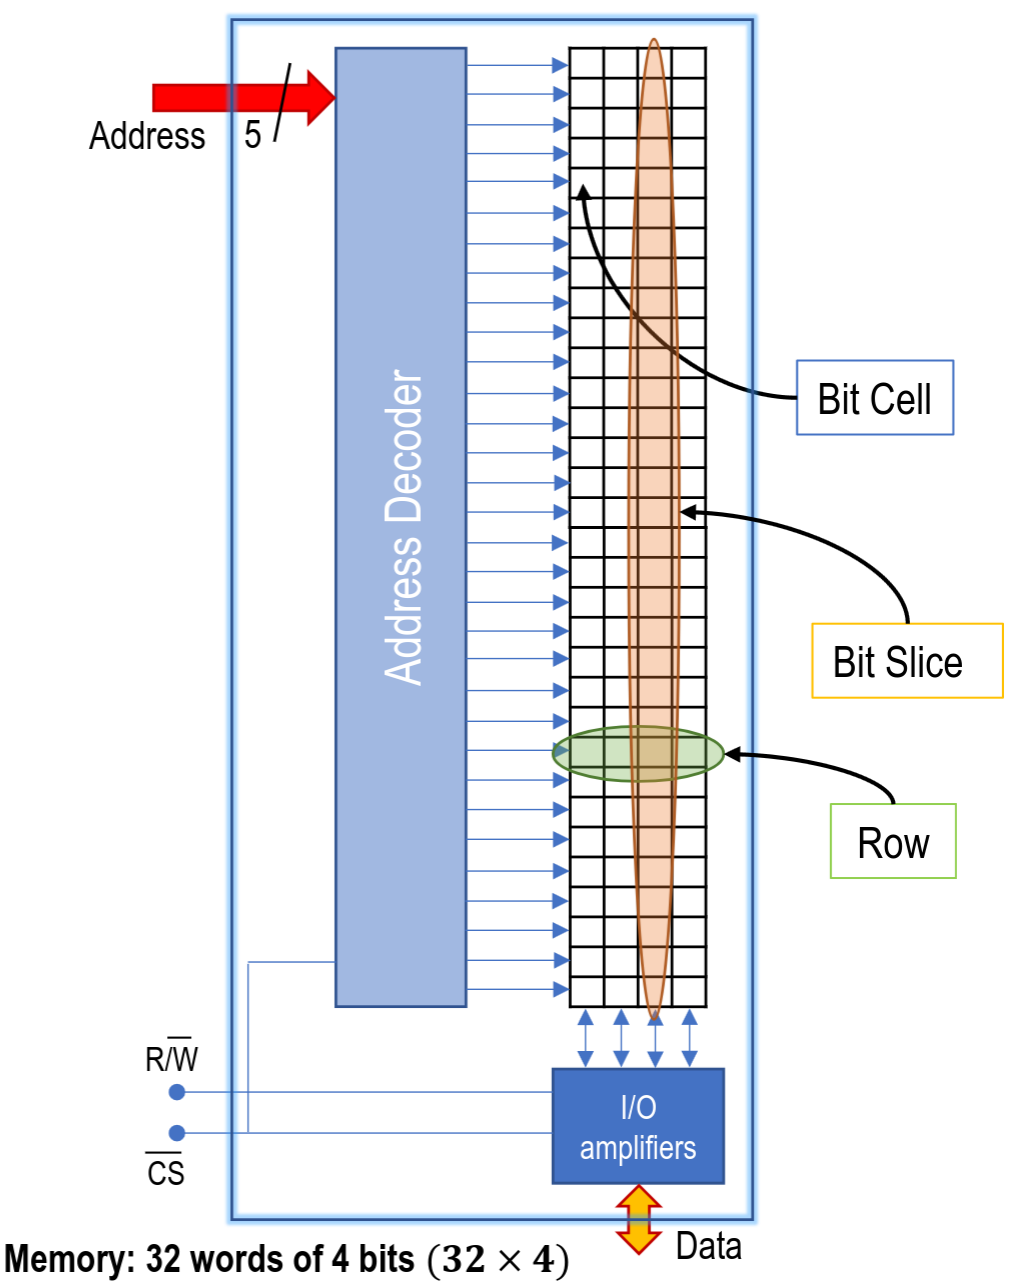
\includegraphics[scale=0.3]{../figures/mem_logi.png}
\end{center}

Some \textit{address decoder} is used to select a single row of the memory: from $k$ address lines to $2^k$ word select lines.
At the word interface, a sense amplifier and I/O circuit are used to interface to the external world.

This is not the ideal approach though, as:
\begin{itemize}
	\item The aspect ratio is unusual and difficult to work with;
	\item The size of address decoder is exponential on the number of address bits;
	\item The memory is \textit{slow}: large parasitic capacitance on bit lines increases propagation delays.
\end{itemize}

\subsubsection{Physical structure of digital memories}
We then move on to defining the \textbf{physical} structure of a real memory.
The idea is to not have a \textit{linear}, but a \textbf{square} array (or matrix) of word cells.

\begin{center}
	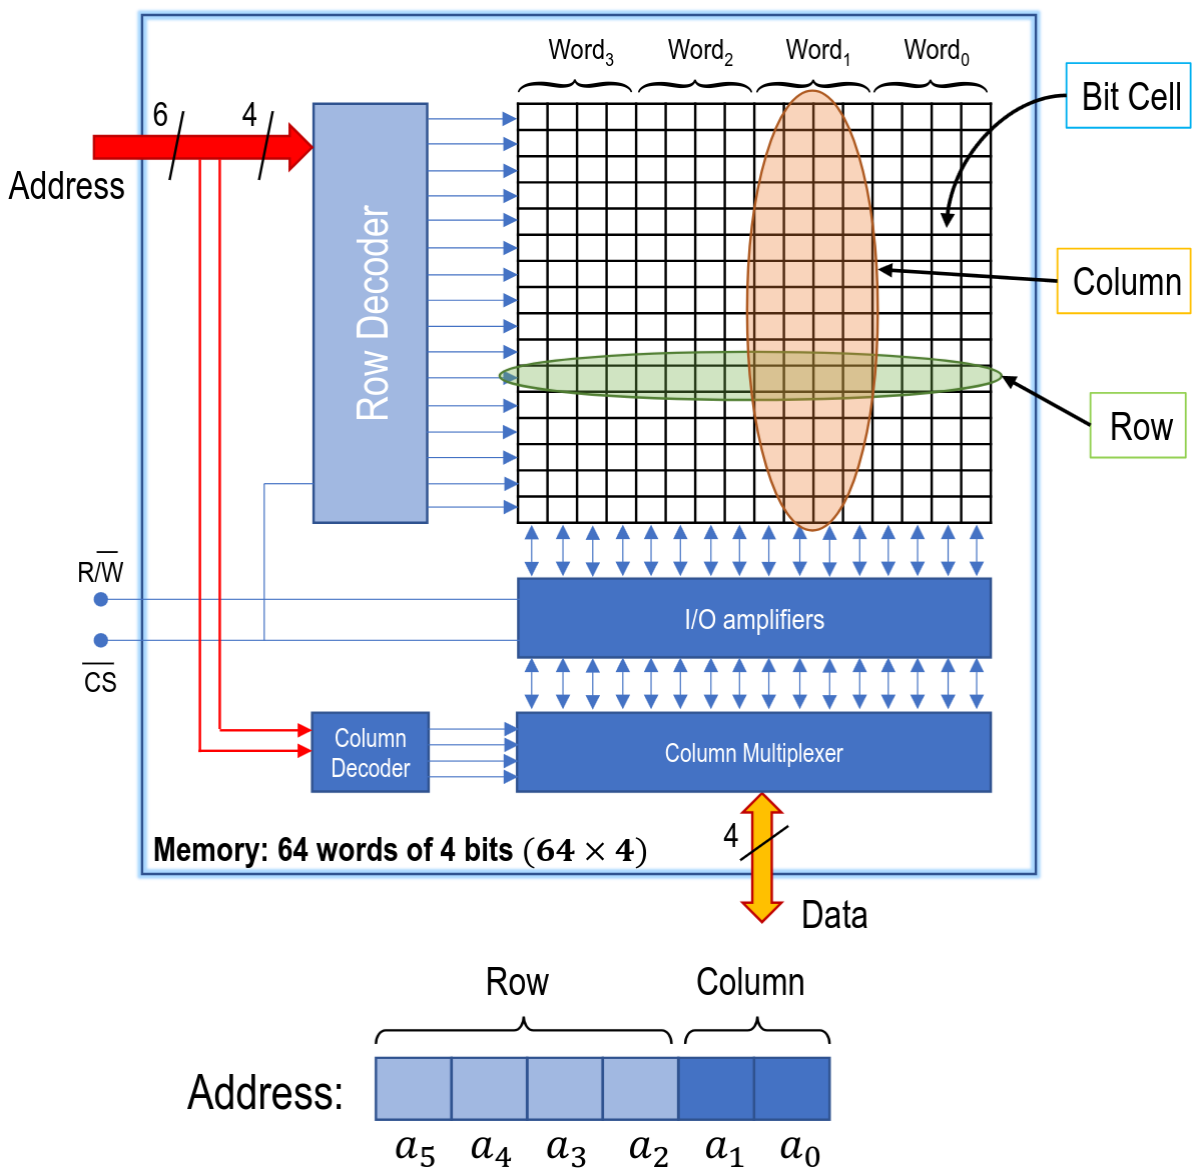
\includegraphics[scale=0.3]{../figures/mem_real.png}
\end{center}

So we find that the real structure is still an array of bit cells, organized in a square array (optimal aspect ratio).
This means that we can have more than one word for each row: one bit slice for each bit in the word, and one column for each word.

Our address decoder has to become a \textit{row decoder}, and we need an additional \textit{column multiplexer} after the I/O amplifiers to select the correct word from a row.
As we can see, this is achieved by splitting the address:
\begin{itemize}
	\item The \textit{upper} side of the address is used to select a row;
	\item Within a row, the \textit{lower} side of the address is used to select a column.
\end{itemize}

The sense amplifier and I/O circuit are still used to interface to the external world.

From the user interface, the interface is the same, but the internal organization is different (and way easier to implement physically).

\subsection{Memory interfaces}

We can now talk about the \textbf{interfaces} of memories.
Usually these are device pins used to access the memory content, write/read it, ...
They are grouped based on their function:
\begin{itemize}
	\item \textbf{Address} bus: identifies the memory location (the index of the word) where an operation is performed. A straightforward address bus is comprised of $k = \log_2(N_\text{words})$ lines;
	\item \textbf{Data} bus: provides the data to/from the memory word. Can be bidirectional, or split in input/output monodirectional buses. A straightforward data bus is comprised of $n_\text{bits}$ lines;
	\item \textbf{Control} bus: this contains the control lines used to perform operations on the data stored in memory. A lot of control lines can be defined, for instance:
		\begin{itemize}
			\item Clock; \item Reset; \item Chip select; \item Output enable; \item Write enable; \item Read/write select; \item ...
		\end{itemize}
\end{itemize}

Memory interfaces (as the name suggests) are designed for interfacing a memory to a digital circuit.
The digital circuit shall connect to all pins of the memory, drive the inputs according to the specifications in the datasheet, and read the outputs.
All of this must be done while complying with the timing diagrams.

\begin{itemize}
	\item In a \textit{custom} digital circuit, the interface is usually designed specifically for the given memory;
	\item In a \textit{standard} digital circuit, there is a generic memory interface: it may require external components to correctly drive a certain memory.
\end{itemize}

\subsubsection{Memory operations}

This can be a good moment to note that the memory \textbf{operations} available are:
\begin{itemize}
	\item Read: given an address, returns the word contained in memory at that address;
	\item Write: Given a word and an address, stores the word in memory at that address;
	\item Match: Given a word, searches the memory for that particular word content and returns the address. This is specific of Content Addressable Memories (\textbf{CAM}, \textit{Content Addressable Memory}, used in caches, for instance);
	\item Erase: initializes the memory to a pre-defined content. Typical of some memories;
	\item Other operations are sometimes available, such as: Burst operation, Partial operation, Precharge, Refresh, ...
\end{itemize}

\subsubsection{Memory protocol}

Data access via the address, data and control lines is performed by an external component on the memory via a predetermined \textbf{protocol}.
he protocol allows organizing the memory to have better performance and area size:
\begin{itemize}
	\item It defines the sequences of signal activations to correctly perform different operations;
	\item It defines the timing constraints.
\end{itemize}

A memory protocol is often described as a timing diagram in the device datasheet.

\subsubsection{Memory composition}

One of the most important concepts regarding memories at the logic level is memory \textbf{composition}.
This entails combining multiple memory chips of a given size $s_i$ to obtain a single addressable memory of size $\sum_i s_i$.

\begin{center}
	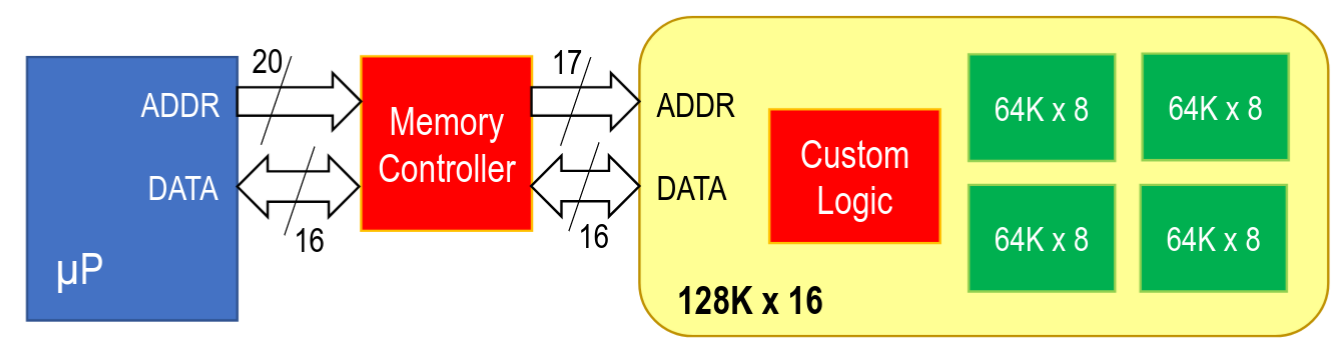
\includegraphics[scale=0.3]{../figures/mem_compo.png}
\end{center}

We have 3 main cases:
\begin{enumerate}
	\item
Let's assume the case where the required memory needs more words than those available in a single memory chip.
For compatibility, we also assume that word width is the same.

This means that addresses are size $k$, with each memory chip having addresses of size $k'$ and:
$$
k > k'
$$

The number of memory chips needed is given by:
$$
n_\text{chips} = \frac{2^k}{2^{k'}} = 2^{k - k'}
$$

We want only one of these chips to be active (to \textit{respond}) for a given address range: this means implementing custom logc to drive the $\overline{CS}$ (\textit{active low Chip Select}) signal of the memory chips.
This custom logic is basically a decoder, controlled by the $k - k'$ additional address lines (over $k'$) and enabling $2^{k - k'}$ (which have to alternatively drive one singular data output bus, a.k.a. tristate outputs).

\begin{center}
	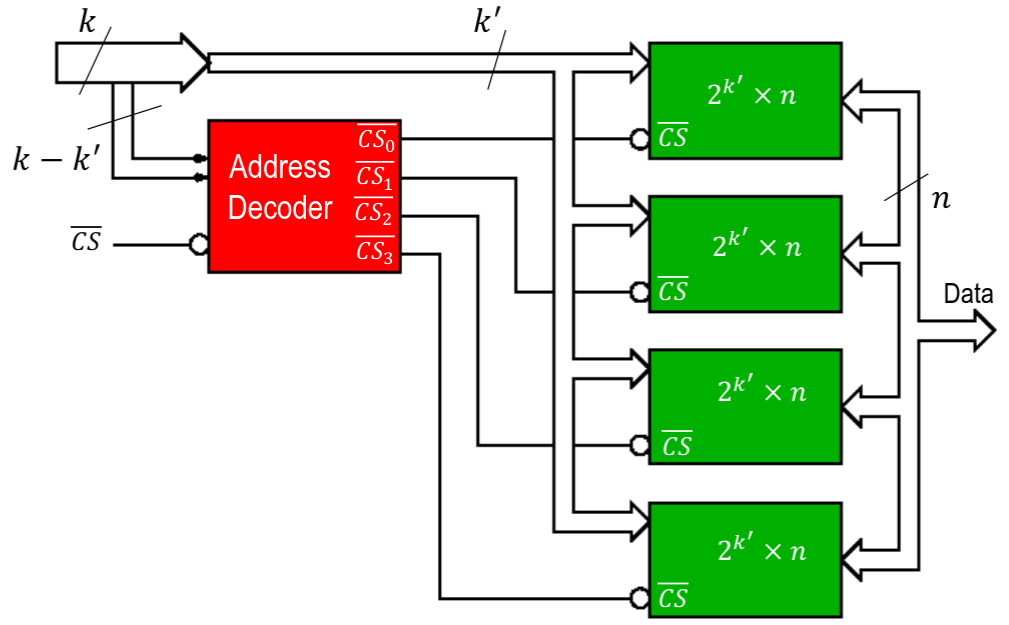
\includegraphics[scale=0.3]{../figures/mem_compo_1.png}
\end{center}

	\item 
Now there's the case where the required memory needs words with more bits than those available on a single memory chip. For compatibility, we also assume that $N_\text{word}$ is the same.

This means that words are to be size $n$, with each memory chip having words of size $n'$ and:
$$
n > n'
$$

The number of memory chips needed is given by:
$$
n_\text{chips} = \mathrm{ceil}\left( \frac{n}{n'} \right)
$$


At this point the composition is trivial:
\begin{itemize}
	\item All memory chips share the same address,;
	\item All memory chips share the same $\overline{CS}$ chip select signal;
	\item Their data busses are combined (concatenated) to form a larger data bus.
\end{itemize}

\begin{center}
	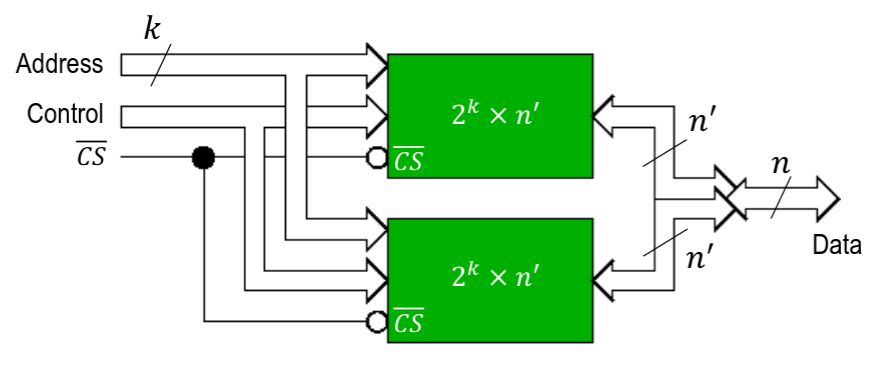
\includegraphics[scale=0.3]{../figures/mem_compo_2.png}
\end{center}

 \item
The last case is the combination of the first two: required memory needs more words than those available in a single memory chip and needs more bits in a word than those available in a single memory chip.

This means that there are:
• $k$ required address lines, but $k$ address lines in a memory chip, with $k > k'$;
• $n$ required data lines, but $n'$ data lines in a memory chip, with $n > n'$.


We need more than one memory chip (of course), and exactly:
$$
n_\text{chips} = \mathrm{ceil}\left( \frac{n}{n'} \right) \cdot 2^{k - k'}
$$

\end{enumerate}

\subsubsection{Memory controllers}

Lastly, let's spend a note on \textbf{memory controllers}.
These can be useful, for instance, when general purpose processors are interfaced with off-the-shelf memory chips: the amount of address lines might not match!

Now in this situation, without a memory controller, the microprocessor accesses the same location in memory with multiple addresses.
Also, some pins are left floating.

A \textit{memory controller} is used to translate addresses and activate the memory.
The memory is mapped to a certain address range in the microprocessor's addressable space: the range does not necessarily start at address $0$: the most significant bits can be used by the memory controller to select the appropriate memory.
Though, it's good to say that the address range is usually aligned to a power of $2$ to simplify the logic.

We know this far too well from our experience with \textit{compiler} tooling: the compiler for the microprocessor should know the chosen address range, so that it generates code that correctly accesses the memory.

Lastly, we note that the memory controller may be integrated inside the microprocessor.

\end{document}
